\documentclass[../main.tex]{subfiles}

\begin{document}
\chapter{Rozwiązywanie równania renderingu}

\section{Wstęp}

Równanie renderingu (ang. \textit{render equation}) zawiera całkę postaci:

\[
  \int_{\Omega} {
    L(\omega_{l})
    f_r(\omega_{v}, \omega_{l})
    \cos \theta_{l}
    d\omega_{l}
  }
\]

Większość obecnie produkowanych silników do gier używa uproszczenia
polegającego na zastosowaniu świateł punktowych, stąd natężenie światła
przychodzącego jest niezerowe tylko w kierunkach będących znormalizowanymi
wektorami między oświetlanym punktem a każdym z aktywnych świateł w scenie.
Powoduje to, że możemy zredukować powyższą całkę do sumy skończonej:

\[ \sum_{l \in L} L(\omega_l) f_r(\omega_v, \omega_l)\cos \theta_l \]

Obliczenie powyższej sumy, nie jest wyzwaniem dla obecnych kart graficznych
nawet dla większej liczby świateł, szczególnie przy zastosowaniu specjalnych
technik zmniejszających wymaganą liczbę operacji do minimum, np.
\textit{deferred shading}.

W przypadku świateł zajmujących ciągły fragment dziedziny sferycznej, całka nie
może zostać w bezpośredni sposób uproszczona do postaci sumy skończonej bez
utraty dokładności. Niestety również dla większośći funkcji $L$, $f_r$
rozwiązanie dokładne nie będzie możliwe do znalezienia w ograniczonym czasie
wymaganym do zachowania płynności aplikacji.

Metody stosujące niebezpośrednie podejście do wyznaczenia przybliżenia wartości
tej całki zostaną opisane w kolenyhch rozdziałach. Wiedza na temat uzyskania
przybliżenia oryginalnej całki przyda nam się do ich zrozumienia oraz
weryfikacji poprawności.

\section{Metoda Monte Carlo}

Całkowanie czynnika równania renderingu:

$$
\int_{\Omega} {
    L_i(l)
    \rho(l,v)
    \cos \theta_{l}
    \: dl
} $$

\noindent nie jest prostym zadaniem do wykonania. Z pomocą przychodzi metoda
przybliona Monte Carlo bazująca na rachunku prawdopodobieństwa i prawie
wielkich liczb. Metoda dokładnie opisana jest w publikacjach
\cite{MonteCarloAnderson}\cite{Veach}.

\vspace{1cm}
\todo[inline]{Definicje zmiennych losowych? Może to przesada.}
\vspace{1cm}

Dystrybuanta (ang. \textit{cumulative distribution function}, \textit{CDF})
wyznacza prawodpodobieństwo, że zdarzenie losowe $\mathbb{X}$, które zachodzi
ma wartość $\eta$ nie przekraczającą $x$.

$$
F(x) = P(\mathbb{X} \leq x)
$$

Funkcją gęstości prawopodobieństwa (ang. \textit{probability density
function}, \textit{PDF}) nazywamy pochodną dystrybuanty:

$$
f_{\mathbb{X}}(x) = \frac{dF}{dx}(x)
$$

Weżmy funkcję gęstości prawdopobieństwa $f_{\mathbb{X}}$ ciągłej zmiennej
losowej $\mathbb{X}$. Wartość oczekiwana funkcji $g$ na ciągłej zmiennej
losowej $\mathbb{X}$ wynosi:

$$
\mathbb{E}(g(x)) =
\int_{\mathbb{X}}{
  g(x) f_{\mathbb{X}}(x)
  \: dx
}
$$

Estymatorem Monte Carlo przybliżającym wartość $\mathbb{E}(g(x))$ opartym na
prawie wielkich liczb nazywamy:

\[
\widetilde{g_n}(x) =
  \frac{1}{n}
  \sum_{i=1}^{n}g(x_i)
\]

\noindent gdzie, $x=(x_1, \ldots, x_n)$ jest zbiorem $n$ próbek zmiennej
losowej $\mathbb{X}$.

\section{Generowanie próbek}

Próbki Monte-Carlo można wybierać w sposób całkowicie losowy (rys.
\ref{fig:RandomSamples}, jednak taka metoda nie daje nam żadnej gwarancji, że
wybrane próbki będą pokrywały dziedzinę w sposób równomierny. Z pomocą
przychodzą nam ciągi \textit{quasi-losowe}, które pokrywają zadaną dziedzinę w
sposób całkowity i równomierny. Załóżmy, że nasza dziedzina jest kostką $n$
wymiarową: $[0,1]^{n}$.

\begin{figure}[h]
  \centering
  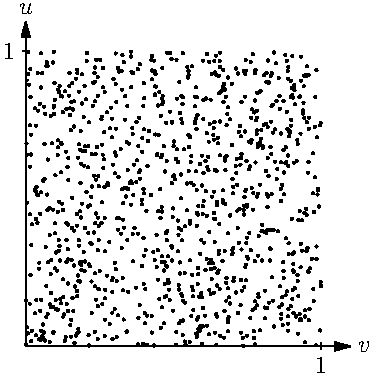
\includegraphics[height=5cm]{montecarlo/random_seq.pdf}
  \caption{Próbki wygenerowane w sposób losowy (1024 próbek)}
  \label{fig:RandomSamples}
\end{figure}

Pierwszą metodą jednorodną jaka się narzuca jest zbudowanie równomiernej siatki
posiadającej $m$ punktów na boku kostki. Problemem tej metody jest jej zbyt
duża jednorodność, wybrane punkty są ułożone w bardzo precyzyjny sposób. Drugim
problemem w niektórych aplikacjach jest ograniczoność metody, zdefiniowaliśmy
dokładnie $m^{n}$ punktów, które musimy wykorzystać, aby zbiór mógł być uważany
za jednorodny, nie możemy punktów usuwać ani dodawać.

\begin{figure}[h]
  \centering
  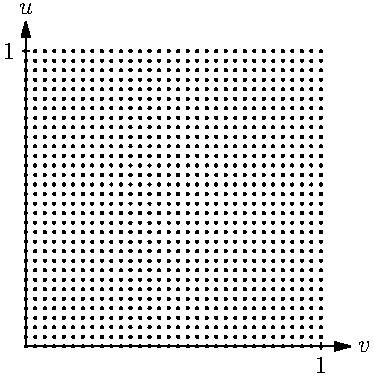
\includegraphics[height=5cm]{montecarlo/uniform_seq.pdf}
  \caption{Próbki wygenerowane przez równomierny podział (1024 próbek)}
  \label{fig:UniformSamples}
\end{figure}

Ciągi o niskiej rozbieżności są rozwiązaniem tego problemu, są to ciągi
deterministyczne, które wydają się losowe przez co posiadają ich zalety oraz
pokrywają równomiernie całą dziedzinę niezależnie od wybranej ilości punktów.

Najbardziej znanymi ciągami tego typu jest ciąg \textit{van der Corput'a} oraz
jego pochodne czyli ciąg Haltona, zbiór Hammersleya.

\subsection{Ciąg van der Corput'a}

Ciąg van der Corput'a \cite{WongSamplingWH} jest jednowymiarowym ciągiem o
niskiej rozbieżności zdefiniowanym na zbiorze $[0,1]$ zbudowanym poprzez
odwrócenie bazy reprezentacji w danym systemie o podstawie $b$. Każda liczba
całkowita $i$ może zostać przedstawiona w pewnej zadanej bazie w sposób
następujący:

\[ i = \sum_{j=0}^{\infty} {a_j b^j} \]

Ciąg van der Corputa transformuje powyższą reprezentację $a_k$, dla $n$-tego
elementu ciągu mamy:

\[ v(n) = \sum_{j=0}^{\infty} {a_j b^{-j-1}} \]

\begin{example}

  Weźmy liczbę $7$ i bazę $2$. Reprezentacja tej liczby może zostać rozpisana
  jako (bez zer nieznaczących):

  \[ 7 = 1 * 2^0 + 1 * 2^1 + 1 * 2^2 = (111)_{b} \]

  \noindent Zatem:

  \[
    v_{2}(7)
      = \frac{1}{2^{1}} + \frac{1}{2^{2}} + \frac{1}{2^{3}}
      = \frac{1}{2} + \frac{1}{4} + \frac{1}{8}
      = 0.875
      \in (0,1)
  \]

\end{example}

Warto zauważyć, że $\sum_{n=1}^{\infty} \frac{b-1}{b^n} = 1$ dla $b>1$.

Kod realizujący powyższe zadanie może być zapisany w formie:

\begin{lstlisting}[language=c++]
float VanDerCorput(unsigned int n, unsigned int base) {
  auto denominator = 1.0f;
  auto result = 0.0f;

  while (n > 0) {
    denominator /= base;
    result += denominator * (n % base)
    n /= base;
  }

  return result;
}
\end{lstlisting}

Istnieje alternatywne rozwiązanie korzystające z właściwości operacji takiej
odwrotności. Warto zauważyć, że obie liczby $n$ oraz $v(n)$ zapisane binarnie
są odbiciem lustrzanym:

\[
  5 = 1 + 4 = (101.0)_{b} \quad
  (0.101)_{b} = 0.625 = \frac{1}{2} + \frac{1}{8} = v(5)
\]

Odpowiednio skonstruowana operacja bitowa tego typu pozwoli na uzyskanie
poprawnego wyniku i zwiększenie wydajności obliczeń \cite{dammertz_2012}.

\subsection{Ciąg Haltona}

Ciąg Haltona jest uogólnieniem ciągu \textit{van der Corput}'a do wyższych
wymiarów. Weźmy $n$ wzajemnie względnie pierwszych liczb $b_i$ większych od 1,
czyli takiego zbioru w którym dla dowolnej pary liczb ich jedynym wspólnym
dzielnikiem jest 1.

$i$-ty $n$-wymiarowy element ciągu Haltona równy jest:

\[ x(i) = \left( v_{b_0}(i), v_{b_1}(i), \cdots, v_{b_n}(i) \right) \]

\begin{figure}[h]
  \centering
  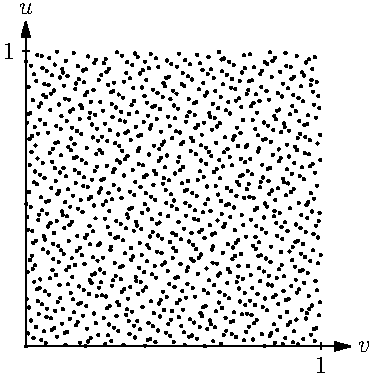
\includegraphics[height=5cm]{montecarlo/halton_seq.pdf}
  \caption{Ciąg Haltona (1024 próbek)}
  \label{fig:HaltonSamples}
\end{figure}

\subsection{Zbiór Hammersleya}

Zbiór Hammersleya jest ciągiem bardzo podobnym do ciągu Haltona, również
korzystającym z ciągu van der Corputa. Chcemy wygenerować $m$ punktów, weźmy
$n-1$ wzajemnie względnie pierwszych liczb $b_i$ większych od 1. $i$-tym $n$
wymiarowym elementem ciągu jest:

\[
  x(i) = \left(
    \frac{i}{m}, v_{b_0}(i), v_{b_1}(i), \cdots, v_{b_{n-1}}(i)
  \right)
\]

\begin{figure}[h]
  \centering
  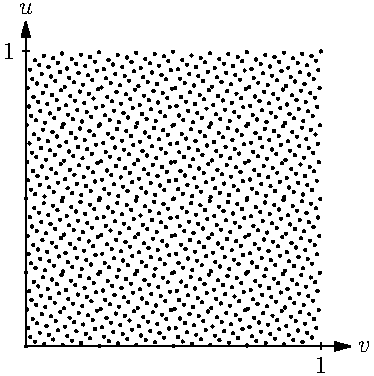
\includegraphics[height=5cm]{montecarlo/hammersley_seq.pdf}
  \caption{Zbiór Hammersleya (1024 próbek)}
  \label{fig:HammersleySamples}
\end{figure}

\subsection{Generowanie punktów na sferze}

Do wygenerowania punktów na sferze możemy wykorzystamy parametryzację:
  $(u,v) \in [0,1]^2 \rightarrow (\theta, \phi) \in \mathbb{H}$

Możemy wykorzystać do tego parametryzację jednorodną \cite{dammertz_2012}:

\begin{align*}
	\phi &= \cos^{-1}(1-u) \\
	\theta &= 2 \pi v
\end{align*}

Lub przekształcenie kosinusowe:

\begin{align*}
  \phi &= \cos^{-1}(\sqrt{1-u}) \\
  \theta &= 2 \pi v
\end{align*}


\section{Przyrostowa metoda Monte-Carlo}

Metoda Monte-Carlo ze względu na swoją złożoność obliczeniową nie umożliwia
uzyskania rezultatu w czasie rzeczywistym. Możliwość operowania sceną,
precyzyjnego ustawienia kamery i obiektów nie jest łatwe w takim środowisku.
Czasami nie potrzebujemy również bardzo dużej szczegółowości, czasem wystarczy
nam konkretna ilość iteracji do znalezienia problemu i głównych różnic.

Wygodnym kompromisem jest podzielenie obliczeń na wiele etapów, z których każdy
może zostać wyświetlony jako częściowy podgląd. Dłuższy czas oczekiwania bez
zmian w scenie pozwala nam uzyskać większą jakość.

Spróbujmy zbudować ciąg podsum Monte-Carlo:

\[ I_n = \frac{1}{n} \sum_{i=1}^{n} f(x_i) \]
\[
  I_{n+1} = \frac{1}{n+1} \sum_{i+1}^{n+1}f(x_i)
    = \frac{n}{(n+1)n} \sum_{i=1}^{n}f(x_i) + \frac{1}{n+1}f(x_{n+1})
    = \frac{n}{n+1} I_{n} + \frac{1}{n+1}f(x_{n+1})
\]

Dodatkowy czas potrzebny na przygotowanie ramki, policzenie sumy ważonej i
wyświetlenie rezultatu na ekranie sprawia, że uzyskamy szybszą zbieżność przez
zgrupowanie próbkek w pakiety, które mogą zostać potencjalnie policzone
jednocześnie. Okazuje się, że rozpisanie analogicznego równania dla paczek
danego, stałego rozmiaru jest trywialne:

\begin{align*}
  I_{(m+1)n} &= \frac{1}{(m+1)n} \sum_{i=1}^{(m+1)n} f(x_i)
  = \frac{1}{(m+1)n} \sum_{i=1}^{mn} f(x_i)
    + \frac{1}{(m+1)n} \sum_{i=mn+1}^{(m+1)n} f(x_i) = \\
  &= \frac{m}{(m+1)mn} \sum_{i=1}^{mn} f(x_i)
    + \frac{1}{(m+1)n} \sum_{i=mn+1}^{(m+1)n} f(x_i) \\
  &= \frac{m}{m+1}I_{mn}
    + \frac{1}{m+1} \left(
        \frac{1}{n} \sum_{i=mn+1}^{(m+1)n} f(x_i)
    \right)
\end{align*}

Powyższe obliczenie sumy ważonej może zostać zrealizowane za pomocą sprytnie
zbudowanego łańcucha \textit{framebufferów} i obliczone za pomocą wspartego
sprzętowo mechanizmu łączenia kolorów (ang. \textit{blending}). Obecna partia
musi zostać obliczona do jednego z buforów oraz skopiowana z włączonym
mieszaniem kolorów do drugiego bufora. Można zastosować uproszczenie, w którym
wykorzystamy tylko jeden bufor, ale czasami ze względu na istnienie wielu
świateł i wybraną technikę (np. \textit{deferred shading}) może być koniecznie
zastosowanie dwóch buforów.

\section{Importance Sampling}

Importance Sampling jest jedną z metod ograniczania wariancji metody
Monte-Carlo. Innymi słowy, zastosowanie tej techniki poprawnie powinno
skrócić czas w którym ciąg zbiegnie do odpowiednio bliskiej wartości całki.

Publikacje \cite{Veach}\cite{MonteCarloAnderson} sugerują zastosowanie innej
techniki generowania próbek, tak aby większość z nich była generowana w
miejsach które są istotne dla wyniku.

Mając funkcję gęstości zmiennej losowej $\mathbb{X}$ $h(x)$ na której potrafimy
całkować, wyznaczać jej wartość w punkcie oraz jest prawie proporcjonalna do
całkowanej funkcji $g(x)$ możemy przepisać:

\[
  \int_{x \in \mathbb{A}} { g(x) dx } =
  \int_{x \in \mathbb{A}} { g(x) \frac{h(x)}{h(x)} dx } =
  \int_{x \in \mathbb{A}} { \frac{g(x)}{h(x)} h(x) dx } =
  \mathbb{E}\left({ \frac{g(x)}{h(x)} }\right)
\]

Aby funkcja $h(x)$ była użyteczna, musi spełniac kilka warunków:

\begin{itemize}

  \item obliczenia dotyczące funkcji $h$ muszą być łatwo realizowalne,
    obliczenie wartości funkcji, jej całki musi być możliwe bez wykorzystania
    metody Monte-Carlo

  \item symulowanie próbek z rozkładu $h$ musi być realizowalne

  \item $h(x) > 0$ dla $g(x) \neq 0$

  \item $h(x)$ musi być możliwie proporcjonalne do $|g(x)|$, inaczej wariancja
    zamiast zmaleć, wzrośnie

\end{itemize}

\section{Multiple Importance Sampling}

\cite{pbrt}

\subsection{Multi-sample model}

\[
  F = \sum_{i=1}^{n} \frac{1}{n_i} \sum_{j=1}^{n_i} w_{i}(X_{i,j}) \frac{
    f(X_{i,j})
  }{
    p_{i}(X_{i,j})
  }
\]

\subsection{Balance heuristics}

\[
  w_{i}(x) = \frac{
    n_{i} p_{i}(x)
  }{
    \sum_{k} {
      n_{k} p_{k}(x)
    }
  }
\]

\end{document}
